\documentclass[12pt]{article}                                                                                                                       
\usepackage{sbc-template}                                                 
\usepackage{graphicx,url}                                                 
\usepackage[utf8]{inputenc}                                               
\usepackage[brazil]{babel}                                                      

\title{Religiões do Mundo\\O Islã}
\author{Iyan Lucas Duarte Marques\inst{1}
Matheus Costa Faria\inst{1}
Camila Moreira Lopes\inst{1}\\
Carlos Henrique Cury Ferreira Lima\inst{1}
Matheus Trindade Rocha\inst{1}}

\address{Instituto de Ciências Exatas e Informática - Pontifícea Universidade Católica Minas Gerais (PUC-MG)}

\begin{document}

\maketitle
\section{Introdução}
O Islã é uma religião do tronco judaico originária na península arábica com a suas figuras centrais, o profetá maior Muhhamed e o único deus do panteão, Alá.
Atualmente, a religião é segmentada por três grandes escolas, a Sunita, a Xiita e a Ibadi. 
Cada escola possui também as suas ramificações com interpretações próprias do livro sagrado Alcorão, adquirindo um caráter descentralizado, ou seja, sem uma figura líder central na religião.
Desta forma, o Islã não possui uma instituição forte como o ramo cristão.
Os muçulmanos acreditam que Alá é único e incomparável e o propósito da existência é adorá-lo.
Eles também acreditam que o Islã é a versão completa e universal de uma fé primordial que foi revelada em muitas épocas e lugares anteriores, incluindo por meio de Abraão, Moisés e Jesus, que eles consideram profetas.
Os seguidores do Islã afirmam que as mensagens e revelações anteriores foram parcialmente alteradas ou corrompidas ao longo do tempo, mas consideram o Alcorão como uma versão inalterada da revelação final de Alá.
A maioria dos muçulmanos vivem majoritariamente na África e sul da Ásia, des do Magarebe às ilhas malacas.
\section{Origem/matriz cultural}
\subsection{Fundador}
O início do Islã ocorre com o ultimo profeta\footnote{
    O profeta Mohammad (ou Maomé), é considerado o último da série de profetas que o mundo teria.
    Baseado nos textos islâmicos, Alá enviou vários profetas para guiar a humanidade, entre eles, Jesus, Abraão, Moisés.
}Maomé, mercador de Meca, recebe revelações de Jibril\footnote{Anjo Gabriel} no ano de 610.
Após a revelação dada por Alá, ele e seus companheiros escreveram o livro sagrado e começaram a pregar pela Arábia.
\par Mohammad viveu os seus últimos 22 anos (ele recebeu as revelações aos 40) pregando a palavra em sua cidade natal, apesar de serem perseguidos pelas autoridades locais.
Após isso, fugiu para a Abissínia convertendo muitos povos locais e escravos.
A elite árabe acreditava que Maomé iria desestabilizar a ordem social através da pregação de uma religião monoteísta, da igualdade racial e do processo de dar ideias aos pobres e seus escravos. 
Depois de 12 anos de perseguição de muçulmanos por os habitantes de Meca, Maomé, sua família e os primeiros muçulmanos realizaram a Hégira ("emigração") para a cidade de Medina (anteriormente conhecida como Iatrebe) em 622.
Lá, com os convertidos de Medina (Ansar) e os migrantes de Meca (muhajirun), Maomé estabeleceu sua autoridade política e religiosa.
\par Um Estado foi estabelecido em conformidade com a jurisprudência econômica islâmica.
A Constituição de Medina foi formulada, instituindo uma série de direitos e responsabilidades para os muçulmanos, judeus, cristãos e para as comunidades pagãs de Medina, unindo-os dentro de uma comunidade - a Umma\footnote{A Umma é um termo islâmico para representar toda a comunidade muçulmana mundial.}.
Após várias peregrinações, batalhas e pregações, Maomé unificou todas as tribos árabes sob o Islã e a Constituição, que dizia:
a segurança da comunidade, a liberdade religiosa, o papel de Medina como um lugar sagrado (com proibição da violência e de armas), a segurança das mulheres, um sistema fiscal para apoiar a comunidade, os parâmetros para alianças políticas exógenas, um sistema de concessão de proteção das pessoas importantes e um sistema judicial para a resolução de litígios em que os não muçulmanos também poderia usar as suas próprias leis. Todas as tribos assinaram o acordo para defender Medina de todas as ameaças externas e de viver em harmonia entre si.
\subsection{Livros sagrados}
O Alcorão\footnote{Do árabe, Recitação} é o livro sagrado da religião islâmica.
Segundo a tradição, é o registro das palavras exatas reveladas por Alá, via intermédio do anjo Gabriel, a Maomé, que o memorizou e ditou aos seus companheiros.
Seu texto é seguido nos dias de hoje por um quarto da população mundial, cerca de 1,3 bilhão de pessoas.
O livro sagrado dos muçulmanos é a própria revelação, a manifestação de Alá.
\par Embora o texto possa soar repetitivo e cansativo em português, em árabe as palavras ganham musicalidade.
Os muçulmanos tem por tradição chamar de Alcorão apenas a versão original, em árabe, com as palavras exatas de Alá, e assim, qualquer outra tradução em geral é denominada “Significado do Alcorão”.
O livro está dividido em 114 capítulos, chamados de suras. Eles [as suras] não contêm uma narração linear.
As suras são organizadas por temas.
Nenhuma palavra de suas 114 suras foi mudada ao longo dos séculos.
Assim, o Alcorão permanece, em cada detalhe, o mesmo livro de quatorze séculos atrás.
\par O Alcorão descreve as origens do Universo, o Homem e as suas relações entre si e o Criador.
Define leis para a sociedade, moralidade, economia e muitos outros assuntos.
Foi escrito com o intuito de ser recitado e memorizado.
Para os muçulmanos, o Alcorão é a palavra de Deus, sagrada e imutável, que fornece as respostas acerca das necessidades humanas diárias, tanto espirituais como materiais.
Ele discute Deus e os seus nomes e atributos, crentes e suas virtudes, e o destino dos não crentes (kuffar); até mesmo temas de ciência.
Os muçulmanos não seguem apenas as leis do Alcorão, eles também seguem os exemplos do profeta, o que é conhecido como a Sunnah, e a interpretação do Corão contida nos ensinamentos do profeta, conhecida como hadith.

\section{Aspectos Simbólicos}
\subsection{Rituais}

\subsubsection{Os Cinco Pilares}
Uma das principais leis sagradas do Islamismo é a Sharia, que significa o caminho que os muçulmanos devem buscar para entrar em sintonia com Deus.  Para isso, os seguidores devem realizar os Cinco Pilares – práticas religiosas voltadas para o desenvolvimento do senso de submissão a Deus. São elas: 
\begin{itemize}
    \item Profissão de Fé: a crença em apenas um deus e no profeta Maomé. 
    \item Preces Rituais: os muçulmanos devem realizar cinco orações diárias (manhã, meio dia, à tarde, início da noite e antes de dormir), de forma coletiva nas mesquitas ou individualmente, contanto que esteja em direção à Meca. 
    \item Doações: contribuição anual dada pelos mais ricos, chamada de Zakat. 
    \item Jejum: no época do Ramadã (nono mês do calendário islâmico), os mulçumanos jejuam durante o dia, exceto crianças, doentes e idosos. O consumo de alimentos e bebidas é liberado ao anoitecer. 
    \item Peregrinação: Pelo menos uma vez na vida os muçulmanos devem peregrinar até Meca (Hadj). Na terra de Maomé, há o compromisso de circular sete vezes em volta da pedra negra, Caaba, localizada no saguão da Mesquita de Al-Haram. 
\end{itemize}
\subsubsection{Peregrinação A Meca}
Todos os muçulmanos que tenham capacidade financeira e saúde devem realizar uma vez na sua vida uma peregrinação à cidade de Meca durante o mês de Dhu al-Hija, mais precisamente entre o oitavo e o décimo-terceiro dia. Se a peregrinação for realizada em outro mês do calendário islâmico, é considerada um ato positivo, mas não corresponde e nem dispensa o Hajj. Em Meca os muçulmanos realizam uma série de rituais, como dar voltas em torno da Caaba.
Jejum
\par Durante o mês do Ramadã, os muçulmanos abstêm-se de comida, de bebida, de fumar, de relações sexuais ou de pensamentos negativos durante o período que decorre entre o amanhecer até ao pôr-do-sol. As pessoas idosas, os doentes e as mulheres grávidas estão dispensadas deste jejum, mas devem realizá-lo em outra altura ou então alimentar pobres durante um período de dias correspondente aos dias que faltaram ao jejum. As crianças também não realizam o jejum. A primeira vez que um muçulmano realiza o jejum funciona como uma espécie de ritual de entrada na vida adulta comparável ao B'nai Mitzvá no judaísmo.
Oração
\par Os muçulmanos devem realizar cinco orações diárias :
\begin{enumerate}
    \item Ao amanhecer.
    \item Depois do meio-dia.
    \item Entre o meio-dia e o pôr-do-sol.
    \item Logo após o pôr-do-sol.
    \item Aproximadamente uma hora após o pôr-do-sol.
\end{enumerate}
Os muçulmanos podem realizar estas orações em qualquer local, desde que este seja um local limpo. É obrigatório virar-se no sentido da cidade de Meca para realizar as orações.
\par Antes da oração, os muçulmanos preparam-se através de abluções, realizadas com água (ou com areia caso não exista água). As partes que são lavadas estão nessa ordem: mãos, boca, inalar a água pelas narinas e soltar-lás pela mesma, o rosto, os braços até a região dos cotovelos, as orelhas, a cabeça e os pés até aos tornozelos, não esquecendo que a ablução é feita três vezes sequências para cada região do corpo citado acima, ex: três vezes as mãos, antes de dar continuidade as outras partes do corpo, começando sempre com o lado direito, menos rosto, orelhas e cabeça que não tem como separar na hora da ablução.
\par As orações devem ser ditas na língua árabe, mesmo que a pessoa não conheça o idioma.
\par A palavra zakat significa purificação e crescimento. Cada muçulmano deve calcular anualmente a sua zakat, que em geral corresponde a 2,5% dos seus rendimentos. As pessoas pobres não precisam pagar zakat, visto que um dos objetivos deste dever religioso é precisamente ajudar os mais pobres. No passado a maior parte dos países muçulmanos cobravam a zakat, mas a prática foi abandonada.

\subsubsection{Rituais Menores}
\begin{itemize}
    \item Nascimento
    Crianças recém-nascidas são saudadas pela comunidade como presentes de Alá. Logo depois do nascimento, o pai do bebê sussurra em seu ouvido direito as palavras do adhan, ou chamado para o oração, e deixa cair um pouco de mel na língua da criança. A cabeça é raspada como símbolo de pureza.
    \item Circuncisão
    Os meninos muçulmanos são circuncidados. Embora não seja mencionado no Corão, esse rito é celebrado desde os tempos bíblicos para simbolizar o pacto entre Deus e os humanos. A circuncisão pode ser feita numa criança desde os oito dias até os dez anos de idade.    
    \item Casamento
    De acordo com um costume local, os casamentos muçulmanos muitas vezes são ajustados entre os pais, que procuram parceiros adequados para seus filhos. O Corão permite que um homem tenha até quatro esposas, mas na prática muitos casamentos muçulmanos são monogâmicos. A cerimônia de bodas pode acontecer na casa da noiva ou do noivo, ou na mesquita. Geralmente é presidida por um imã e inclui leituras do Corão. Há um contrato escrito e o noivo deve pagar um dote pela noiva.    
    \item Morte
    Quando um muçulmano morre, seu corpo é envolvido no ihram e levado até a mesquita para as preces fúnebres. O corpo - que deve ser enterrado o quando antes em respeito ao falecido - é deposto num túmulo simples marcado por um montículo de terra.    
\end{itemize}

\subsection{Papel masculino e Feminino}

\subsubsection{Islã e o princípio de igualdade}
A contextualização da revelação do Islã informa sobre o conteúdo revolucionário de sua mensagem quanto às relações sociais de sexo desiguais, existentes na península arábica do sétimo século da era gregoriana. Essas relações, remanescentes da mentalidade patriarcal e da organização tribal e escravagista da época, relegavam as mulheres ao status de mercadoria, fazendo parte do patrimônio de seu marido e de seus herdeiros.
\par Outras práticas desvalorizaram para as mulheres eram costumeiras na sociedade árabe da época, como a poligamia, que não conhecia nenhuma restrição quanto ao número de esposas, o que dependia unicamente da fortuna e status social do homem, ou o repúdio, o casamento forçado, a privação do direito à herança e a escravidão.
\par A liberação do ser humano – seja ele homem ou mulher – por um lado, de todo tipo de escravidão ou subjugação e, por outro, a reconstrução de relações sociais sobre bases igualitárias, são a base do projeto social inaugurado pela mensagem corânica.
\par O princípio igualitário encontra seus fundamentos no próprio conceito da unicidade de Deus: "Não existe Deus senão Deus", "Nenhum Deus fora de Deus". Essa afirmação constitui uma referência existencial que carrega em si todas as aspirações e/ou reivindicações pela igualdade dos humanos diante de um só Deus, sem nenhum tipo de intermediação. É uma referência liberadora que leva os humanos à sua origem comum:
\par Humanos, Nós vos criamos de um macho e de uma fêmea. Se de vós fizemos povos e tribos, é graças ao seu conhecimento mútuo. O mais digno aos olhos de Deus é aquele que mais se precaver.
\subsubsection{O divórcio}
O divórcio é considerado pelo Islã como "o ato lícito mais detestável aos olhos de Deus" – dito em um hadith, constitui um remédio para uma situação anormal de um casal para o qual a vida em comum se tornaria insuportável. "Se, não alcançando um entendimento, os dois esposos preferem se separar Deus, em sua bondade, lhes dará a cada um, melhor destino".  A dissolução do laço conjugal é um direito que pertence aos dois cônjuges. Quando o marido divorcia-se de sua mulher, ele deve oferecer uma compensação em troca do prejuízo assim sofrido por ela. Por outro lado, a mulher tem o direito de pedir o divórcio e de obtê-lo em caso de prejuízo; na ausência de prejuízo, ela pode obtê-lo através de compensação oferecida ao seu esposo. Nada no Alcorão autoriza um marido a manter a força sua esposa se ela deseja pôr fim à união
\subsubsection{A herança}
O direito sucessório no Islã parte do princípio geral que vê a riqueza como propriedade divina antes de tudo, a qual não deveria ser acumulada como um tesouro, mas dividida igualitariamente entre aqueles que têm direito.
\par A herança no Islã abarca a herança por obrigação subdividida em seis categorias nas quais as partes são definidas da seguinte maneira: os dois terços, a metade, o terço, o quarto, o sexto e o oitavo, e a herança do que sobra uma vez deduzias as partes obrigatórias.
\par Muitas vezes censurou-se o Islã por ter privilegiado em termos de herança o homem ao contrário da mulher, ao conceder ao primeiro o dobro da parte concedida à última – ora, uma análise aprofundada do direito sucessório mostra que essa regra não é aplicada senão em 16,33\% dos casos, e são todos os casos nos quais o homem tem a obrigação de cuidar da família, sabendo-se que a mulher é livre de manter seus bens e não é obrigada a participar das obrigações da casa, mesmo quando ela é rica. No outros casos, ou ela recebe a mesma parte que o homem, ou ela herda uma parte maior – ocorre inclusive que ela o priva totalmente de sua herança.
\subsection{Alá}
Na teologia islâmica, Deus, também reconhecido como Allah (Deus traduzido para árabe) é o onipotente e onisciente criador, mantenedor, responsável e juiz do universo. 
\par O Islã coloca uma grande ênfase na conceitualização de Deus como estritamente singular (tawhid). A unicidade de Deus (Tawhid) é a crença e afirmação de que Deus é um e único. O alcorão assegura a existência de uma única e absoluta verdade que transcende o mundo; um único e indivisível ser que é independente de toda a criação. Deus é único (wahid) e inerentemente Um (ahad), misericordioso e onipotente.
	\par De acordo com o Alcorão: “Nenhuma visão pode compreendê-lo, mas sua compreensão está além de toda a visão. Deus está acima de compreensão, mas é inteirado com todas as coisas”. Assim, se dá a entender que Deus existe sem um lugar segundo os ensinamentos islâmicos. Para os mesmo, é dito que a criação e a manutenção da ordem no universo é vista como um ato de misericórdia primordial pela qual todas as criaturas de Deus cantam-lhe glórias e são testemunhas da sua unidade e domínio.
	\par Também se é afirmado que Deus responde aos necessitados ou desafortunados quando eles chamam. Acima de tudo, Deus guia a humanidade para o caminho correto “o caminho sagrado”.
	\par De acordo com a tradição islâmica, há 99 nomes para Deus (al-asma al-husna, “os melhores nomes”), no qual cada um desses evoca um atributo distinto de Deus. Todos estes nomes referem-se a Alá, o nome divino supremo e que tudo compreende. Uma curiosidade é: entre os 99 nomes, os mais famosos e mais usados com frequência são “O Compassivo” (al-rahman) e “O Misericordioso” (al-rahim).
	\par O Islã compreende e ensina que Deus, como referenciado no Alcorão, é o único Deus e o mesmo venerado por membros de outras religiões abraâmicas como Cistianismo e Judaísmo.

\subsection{Mitos originários}
Antes de tudo a mitologia árabe engloba as antigas crenças pré-islâmicas dos árabes. 
\par Antes do Islã na Península Arábica em 622, o centro físico do islã, a Caaba de Meca, estava coberto de símbolos que representam os demônios inumeráveis, djinn, semideuses e outras criaturas sortidas que representava o ambiente profundamente politeísta pré-islâmica da antiga Arábia. Podemos inferir a partir desta pluralidade um contexto excepcionalmente amplo em que a mitologia pode florescer.
\par Histórias de gênios, ghouls, lâmpadas mágicas, tapetes voadores, e os desejos contidos nos contos das Mil e Uma Noites e outras obras foram transmitidos através das gerações.
\par O conceito de mau-olhado é mencionado no Alcorão, em Surat al-Falaq (em que um é contada a procurar refúgio "do mal do invejoso, quando inveja"). A Mão de Fátima é por vezes utilizado para neutralizar o efeito da Evil Eye, embora seu uso é proibido no Islã, como são todos os talismãs e superstições. Entre os muçulmanos tradicionais, vários versículos do Alcorão como uma Nas-e al-Falaq são, por vezes recitado a bênção.

\subsection{Orientações para a Vida e a Morte}
Enquanto vivos aqueles que seguem a religião possuem valores principais em que eles se guiam. O primeiro valor que deve ser seguido é a crença em Alá. Além desse valor principal existem cinco pilares existentes na religião, são eles: Fé, oração, jejum, caridade e peregrinação.
\par Dentro do Islamismo a morte, assim como o nascimento, está nas mãos de Deus, e vivendo de acordo com os ensinamentos divinos, não há motivo para se temer a morte. Acredita-se também que os Islâmicos que morrem em jihad vão direto para o paraíso.
\subsection{Valores}
Os seguidores da religião se apoiam e compartilham um conjunto de crenças fundamentais, essas que possuem 6 principais tópicos, são eles:
\begin{itemize}
    \item Crença em um Deus único
    \item Crença nos anjos
    \item Crença nos profetas de Alah
    \item Crença no dia do juízo
    \item crença no destino e no Decreto Divino
\end{itemize}

\section{O Islã no Brasil}
\subsection{Adeptos:}
O censo de 2010, realizado pelo IBGE, apontou a existência de apenas 35.167 muçulmanos no Brasil, mas existem dados que apontam cerca de 1,5 milhão de pessoas muçulmanas no país.
Após a Primeira Guerra Mundial, diversos árabes se mudaram para o Brasil.Com isso, no ano de 1927, foi criada a Sociedade de Bem-Estar Palestina Muçulmana, na cidade de São Paulo. A partir de 1929, com novos adeptos do Islã chegando ao País, o nome da instituição foi alterado para Sociedade do Bem-Estar Muçulmano.

\begin{figure}[ht]
    % Alterar espaçamentos antes e depois do caption
    \setlength{\abovecaptionskip}{5pt}
    \setlength{\belowcaptionskip}{0pt}
    % Caption
    \caption[Numero de adeptos do Islã no Brasil]
        {Numero de adeptos do Islã no Brasil}
    \centering
    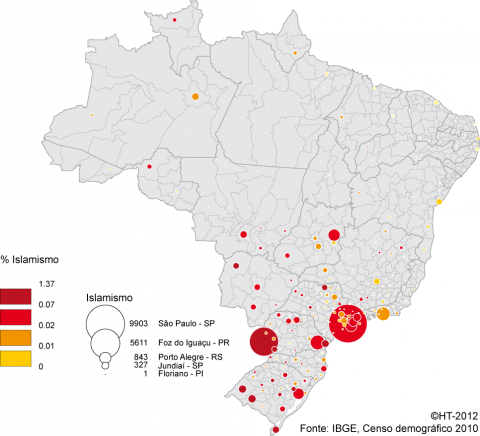
\includegraphics[width=.80\textwidth]{brasil_isla.png}
    % Caption centralizada
    \captionsetup[grafico]{justification=centering}
    % Fonte
    \captionfont{\small{\textbf{\\Fonte: Wikipedia}}}
    \end{figure}

\subsection{Localização:}
 Em todo o País, estima-se que existam oitenta centros do Islã e cerca de 50 mesquitas. As cidades de Foz do Iguaçu, Curitiba, Rio de Janeiro, Brasília e São Paulo abrigam as mais populosas comunidades de muçulmanos no Brasil. Notavelmente, na já citada Foz do Iguaçu, encontra-se o maior número de adeptos da religião. Além da presença de salas destinadas à oração e templos por quase todos os outros Estados que compõem a nação, em São Paulo há aproximadamente 10 mesquitas, sendo que a mais antiga é a Mesquita Brasil, fundada no continente latino-americano a partir do ano de 1929.

\section{O Islã no Mundo}
 \subsection{Adeptos:}
 A análise conduzida pelo centro de pesquisa trouxe dados interessantes. Há hoje no mundo 1,6 bilhão de pessoas que se designam muçulmanas.
 \subsection{Localização:}
 Embora o senso comum considere que a maioria dos seguidores dessa religião estejam no norte da África ou no Oriente Médio, apenas 20% deles encontram-se nesses lugares. A maioria dos muçulmanos (62%) está na região Ásia-Pacífico. O maior país muçulmano é a Indonésia. Pelo menos nos dias atuais: em 2050, calcula o estudo, o país com a maior comunidade islâmica do mundo será a Índia, que hoje tem como maior grupo religioso o hindu.

 \begin{figure}[ht]
    % Alterar espaçamentos antes e depois do caption
    \setlength{\abovecaptionskip}{5pt}
    \setlength{\belowcaptionskip}{0pt}
    % Caption
    \caption[Numero de adeptos do Islã no Mundo]
        {Numero de adeptos do Islã no Mundo}
    \centering
    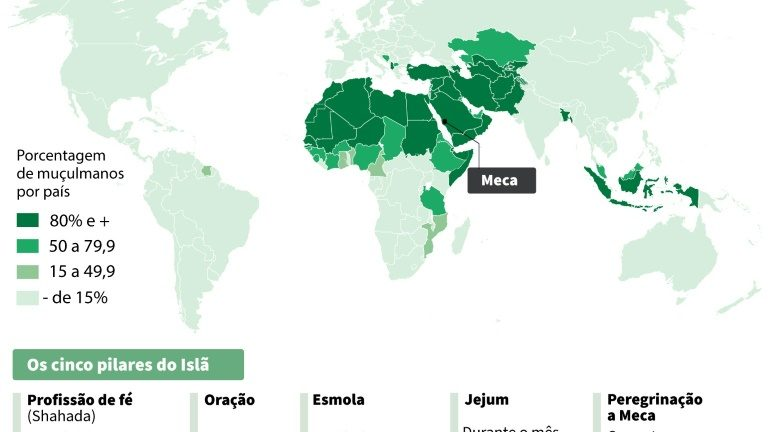
\includegraphics[width=1.10\textwidth]{mundo_isla.png}
    % Caption centralizada
    \captionsetup[grafico]{justification=centering}
    % Fonte
    \captionfont{\small{\textbf{\\Fonte: Wikipedia}}}
    \end{figure}

\end{document}